
\section{Referanselister}

	\begin{frame}{Referanselister}
	
	Skikkelige referanselister er både viktig for å unngå plagiat, og nyttig for å hjelpa lesaren til å finna meir informasjon. \LaTeX har fleire system for å automatisera delar av jobben med innhenting av metadata, og generering av referanselister:
	
	\begin{itemize}
		\item BibTeX
		\item BibLaTeX
	\end{itemize}
	
	BibLaTeX er det moderne alternativet til BibTeX og er det ein bør nytta.
	
\end{frame}





\begin{frame}[containsverbatim]
	
	Referanselister i \LaTeX{} kan manuelt leggast inn på fylgjande måte:
	
	\begin{minted}[breaklines]{latex}
\begin{thebibliography}{9}
	\bibitem{texbook}
	Donald E. Knuth (1986) \emph{The \TeX{} Book}, Addison-Wesley Professional.
	
	\bibitem{lamport94}
	Leslie Lamport (1994) \emph{\LaTeX: a document preparation system}, Addison
	Wesley, Massachusetts, 2nd ed.
\end{thebibliography}
	\end{minted}
	
\end{frame}


\begin{frame}[containsverbatim]{Referanselister}
	
	Som gir resultatet:
	
	\begin{thebibliography}{9}
		\bibitem{texbook}
		Donald E. Knuth (1986) \emph{The \TeX{} Book}, Addison-Wesley Professional.
		
		\bibitem{lamport94}
		Leslie Lamport (1994) \emph{\LaTeX: a document preparation system}, Addison
		Wesley, Massachusetts, 2nd ed.
	\end{thebibliography}
	
	Teksten kan referera til referansane ved hjelp av ``cite'' kommandoen. Til dømes \mintinline{latex}|\cite{lamport94}|, som gir \cite{lamport94}.
	
	\LaTeX{} \cite{lamport94} er ein pakke med makroar for \TeX{} \cite{texbook}.
	
	\textit{Dette fungerer ikkje saman med den meir avanserte pakken for referanselister som eg nyttar seinare i dokumentet, og ser derfor ikkje riktig ut.}
	
\end{frame}



\begin{frame}[containsverbatim]{Referanselister}
	
	Det er tungvindt å skriva referanselista manuelt. Dei fleste ynskjer å nytta eit verktøy for å organisera alle referansane og å generera lista automatisk.
	
	Ei referanse har ein del metadata som tittel, forfattar, publiseringsdato, ISBN nummer (for bøker), .m.m. Denne informasjonen kan leggast i spesielle *.bib filar som BibLaTeX nyttar for å generera referanselistene. *.bib filane kan ein enten skriva manuelt, ein kan lasta dei ned frå ulike kjelder, eller ein kan nytta ulike verktøy for å generera dei automatisk.	

\end{frame}


\begin{frame}[containsverbatim]{Referanselister}
	
	Oppsettet for ei moderne referanseliste med \textit{biblatex} kan sjå slik ut:
	
	\begin{minted}{latex}
\usepackage[
backend=biber,
style=ieeetr,
sorting=ynt
]{biblatex}
\addbibresource{latex-kurs-referansar.bib}
	\end{minted}
	
	Filen \textit{latex-kurs-referansar.bib} heldt metadata for alle referansane, og er som regel auto-generert.

Kommandoen \mintinline{latex}|\printbibliography| må plasserast der ein ynskjer at referanselista skal plasserast.

\end{frame}


\begin{frame}[containsverbatim]{Referanselister}

Den originale boka om \TeX{} \cite{knuth1986texbook}, og den originale boka om \LaTeX{} \cite{lamport1994latex}.

\printbibliography

\end{frame}


\begin{frame}{Referansehåndtering med Zotero}

  Zotero er eit verktøy for organisering av kjelder og automatisk eksport til *.bib format.

  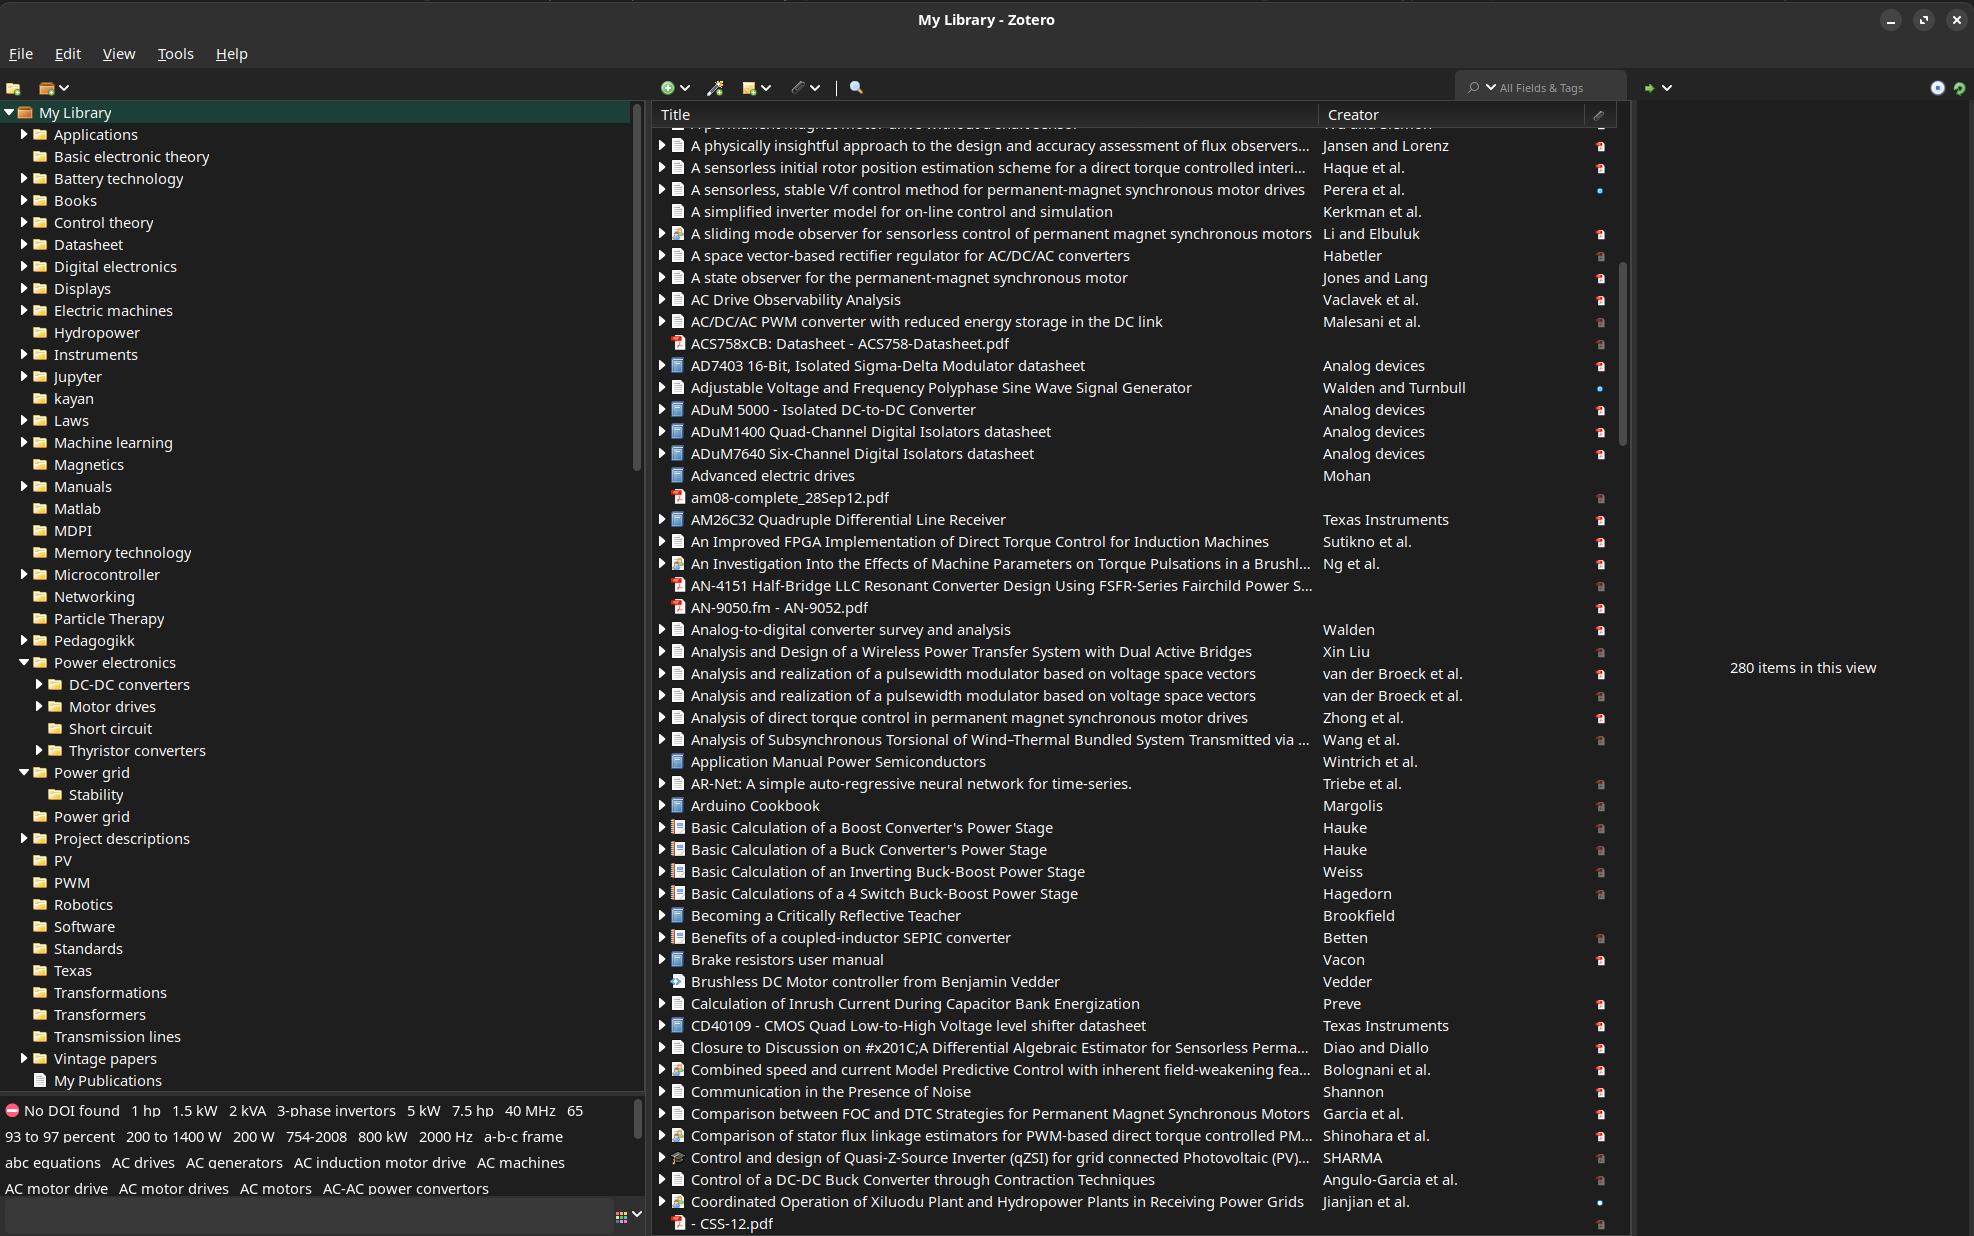
\includegraphics[width=\textwidth]{img/zotero_screenshot.png}
	
\end{frame}

\begin{frame}{Referansehåndtering med Zotero}

  Ein kan setta opp Zotero slik at *bib filen vert holdt oppdatert automatisk når nye referansar vert lagt til, og ein kan dela biblioteket mellom fleire brukarar. For mange nettsider som til dømes IEEE, eller Amazon\footnote{Ikkje bruk Amazon, dei ansatte får ikkje lov å gå på do i arbeidstida.} vil eit tillegg til nettlesaren vera alt du treng for å få alle metadata lagt inn automatisk.
  
\end{frame}

%%% Local Variables:
%%% mode: latex
%%% TeX-master: "../latex-presentation"
%%% End:
